
\chapter{Test phase \#2}\label{ch:test_2}

Pour clôturer la phase de développement \#2 du projet, un test est effectué avec pour objectif de valider que le concept dans son ensemble fonctionne. Ce test a permis de mettre ensemble tous les acteurs du système, le capteur, la passerelle, la base de données et enfin l'application mobile et de vérifier leur bon fonctionnement.

Le test s'est concentré sur la transmission de la position GPS depuis le capteur jusqu'à l'application mobile, les autres éléments du système n'étant pas encore implémentés. L’autre objectif était de vérifier que la mise à jour de la position du coureur se passe bien.

Afin de pouvoir faire ce test, les éléments suivants ont été développés.

\begin{itemize}
\item Firmware du capteur avec l'utilisation de Zephyr et envoi de la position GPS dans un paquet
\item Création de la base de données
\item Implémentation de la réception, décodage et stockage des paquets sur la passerelle
\item Création de la base de l'application mobile avec visualisation des positions GPS sur la carte
\end{itemize}

On comprend que cette phase de développement est représente une part importante du développement complet du projet car tous les composants du système sont développés. Dans un premier temps, seules les fonctionnalités de bases sont implémentées, ce qui permet de s'assurer que toutes les interactions se passent comme prévu avant de poursuivre le travail pour la phase \#3.

Pour le capteur, la base du firmware comprenant le système d'exploitation temps réel Zephyr est mis en place. Pour l'instant il ne fait que de récupérer périodiquement la position GPS grâce au driver $I^{2}C$ implémenté pour l'occasion et l'envoyer dans un paquet LoRa à destination de la passerelle.

Le système PostgreSQL est installé sur la passerelle, puis la base de données est conçue et créée, ce qui permet le stockage des données venant du capteur. Le logiciel serveur d'application est davantage développé afin de pouvoir récupérer les paquets, qui sont d'un format différent que celui du test de la phase \#1, puis grâce à la librairie pqxx, les stocker dans la base.

Le cœur de l'application mobile est écrit, permettant de périodiquement envoyer une requête à la passerelle pour récupérer d'éventuelles nouvelles données et les afficher sur la carte Google maps afin de pouvoir visualiser l'évolution du coureur.

Puisque l'objectif du test est de se mettre dans des conditions réelles, les résultats du test son directement sauvegardés dans la base de données, permettant ainsi de pouvoir consulter toutes les positions facilement depuis l'application mobile. Le téléphone mobile sur lequel s'exécute l'application est connecté à la passerelle grâce à l'access point qui propose et fait les requêtes directement à la passerelle.

Le code utilisé durant ce test correspond au tag de la version v0.2 sur git.

\begin{figure}[htb]
\centering 
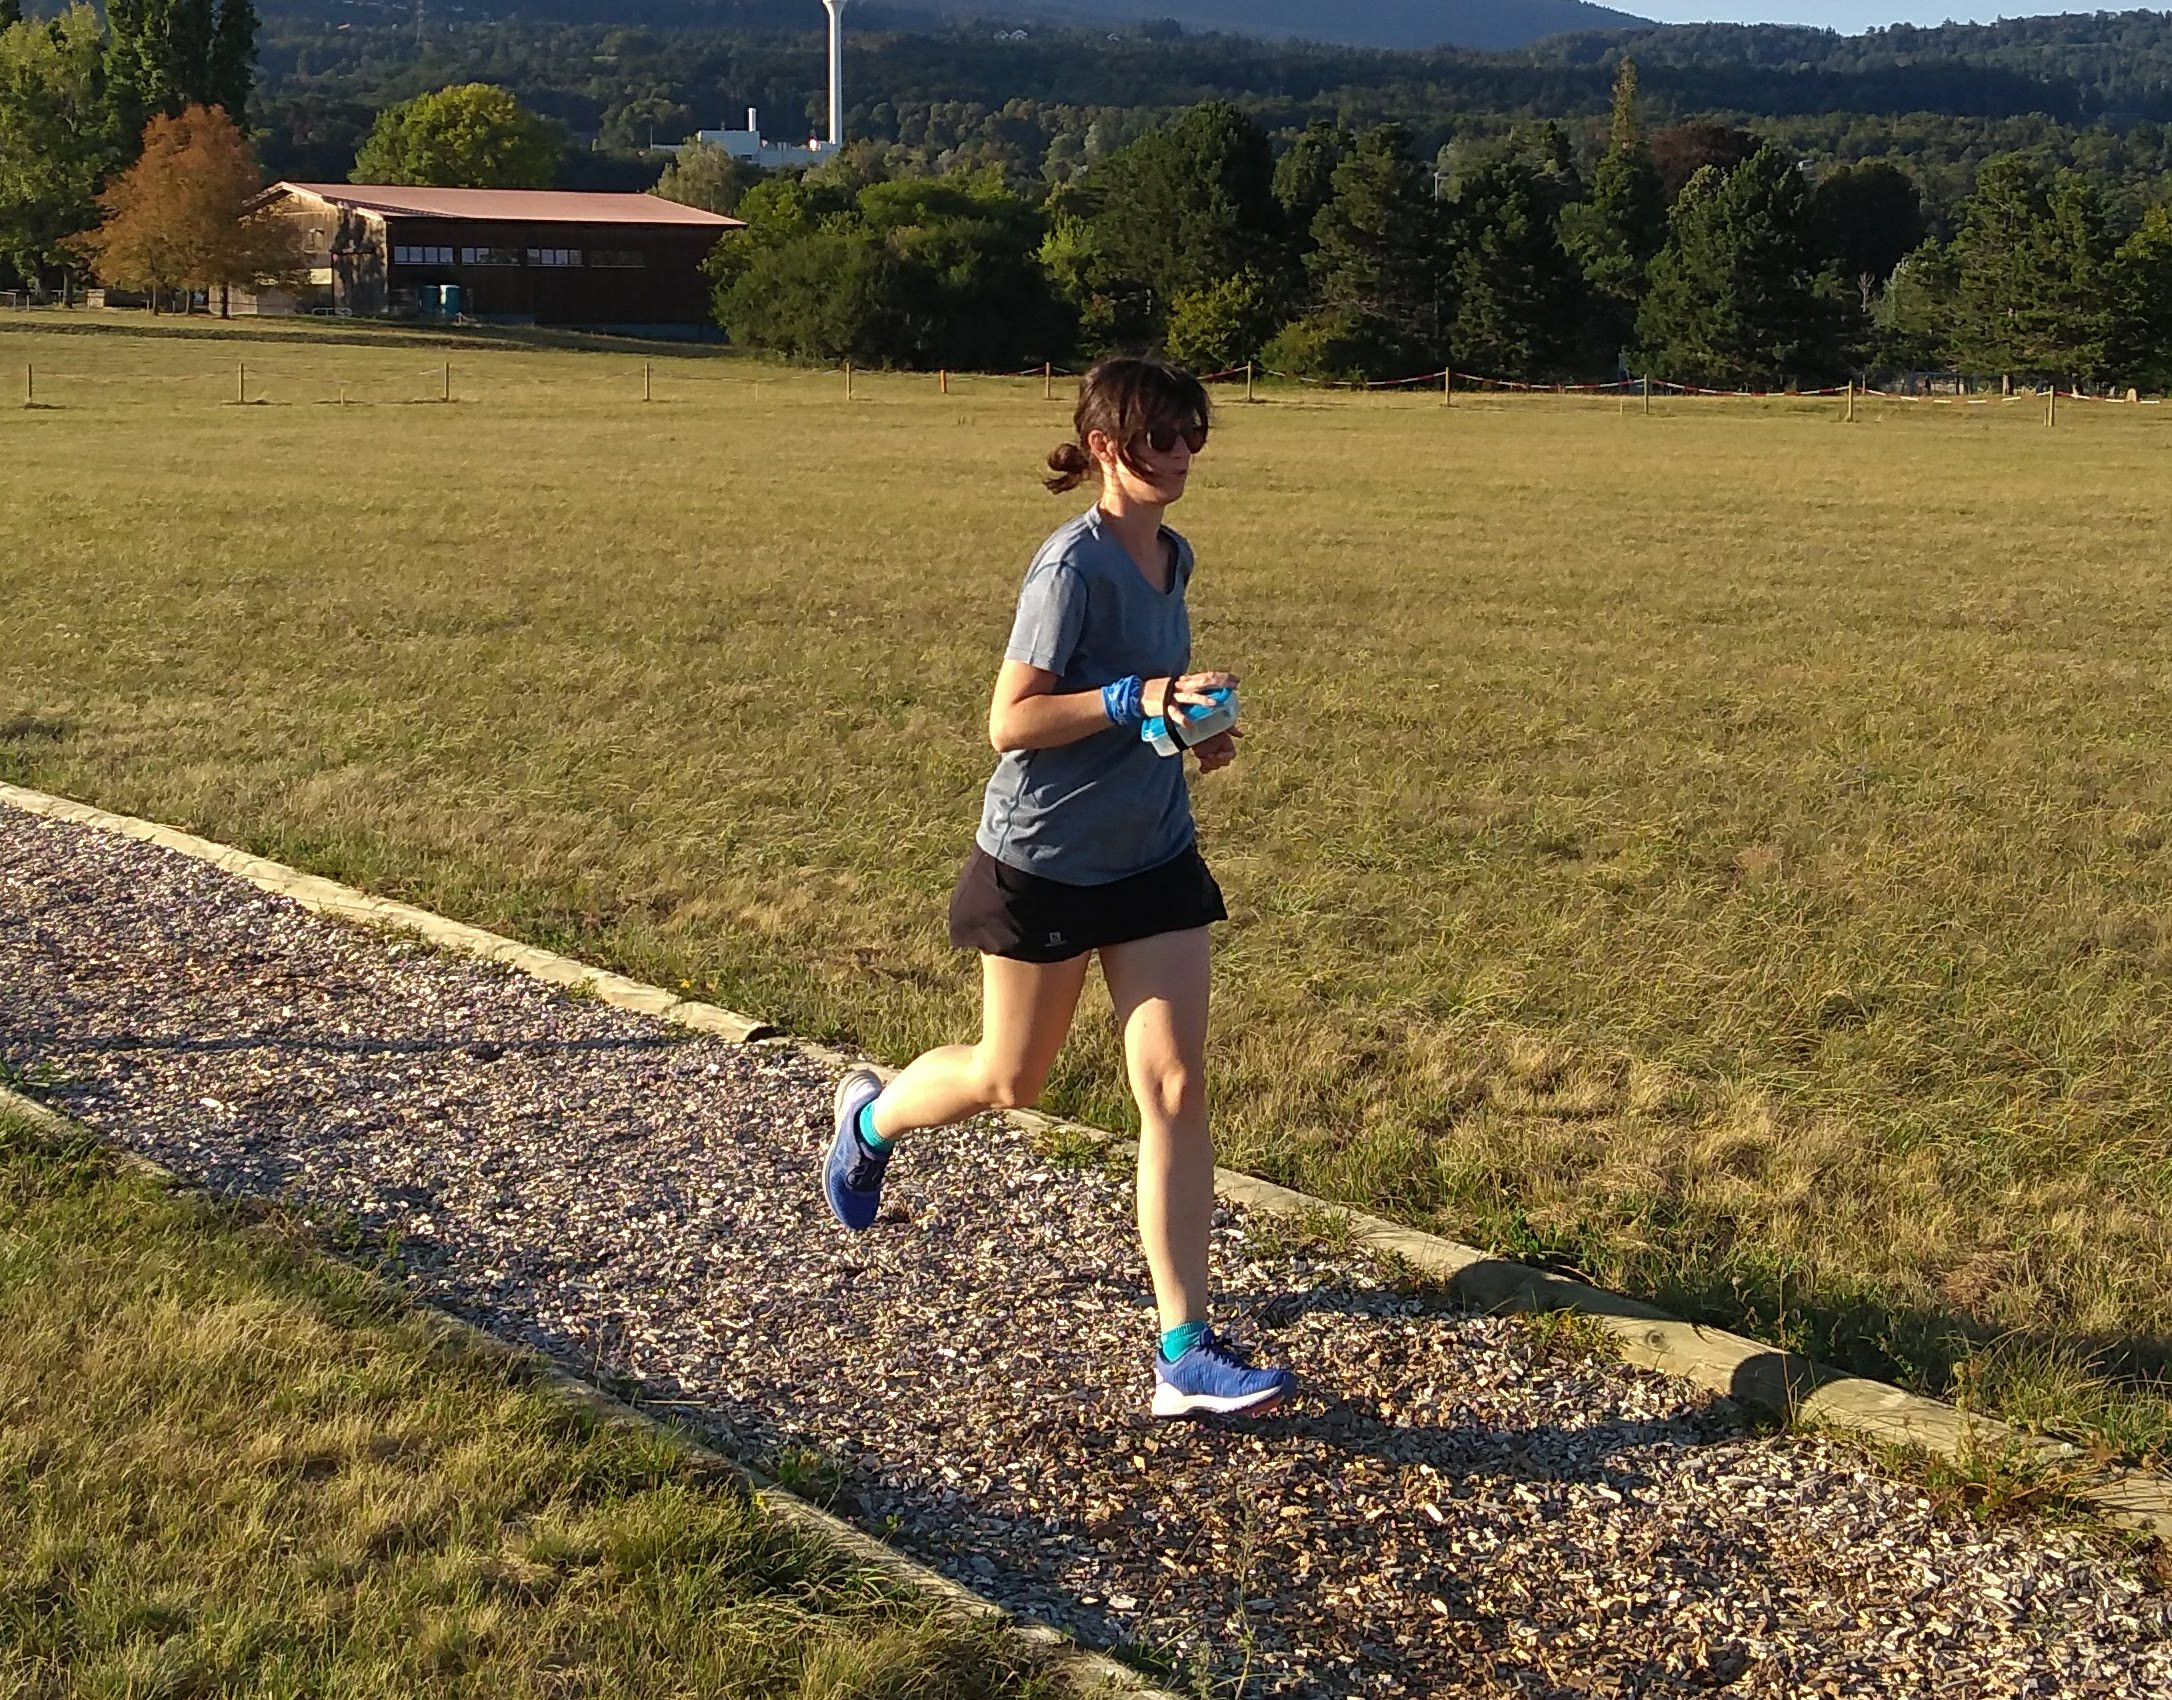
\includegraphics[width=0.7\columnwidth]{running_goo.jpg} 
\caption{Stituation pour le test \#2}
\label{fig:situation_test_2}
\end{figure}

\section{Scénario}

Le scénario de ce test est très simple. Il consiste à recréer les conditions réelles d'utilisation du système. Pour ce faire, un cobaye coureur muni du capteur va courir le long d'un parcours défini afin de vérifier que la position est correctement mise à jour au fil de son évolution.

\section{Résultats}

Après plusieurs échecs dus aux problèmes de connections entre l'application mobile et la passerelle, le test a finalement pu se dérouler sans embuche.

Le test a été effectué le 7 Septembre 2018 sur la piste finlandaise de la place d'arme de Planeyse à Neuchâtel.

Le capteur et la passerelle sont configurés pour utiliser un facteur d'étalement maximal de sf12 afin de s'assurer d'avoir la portée maximum.

Les positions récoltées durant le test peuvent être consultées sur la figure \ref{fig:test_2}.

\begin{figure}[htb]
\centering
\begin{subfigure}{.5\textwidth}
  \centering
  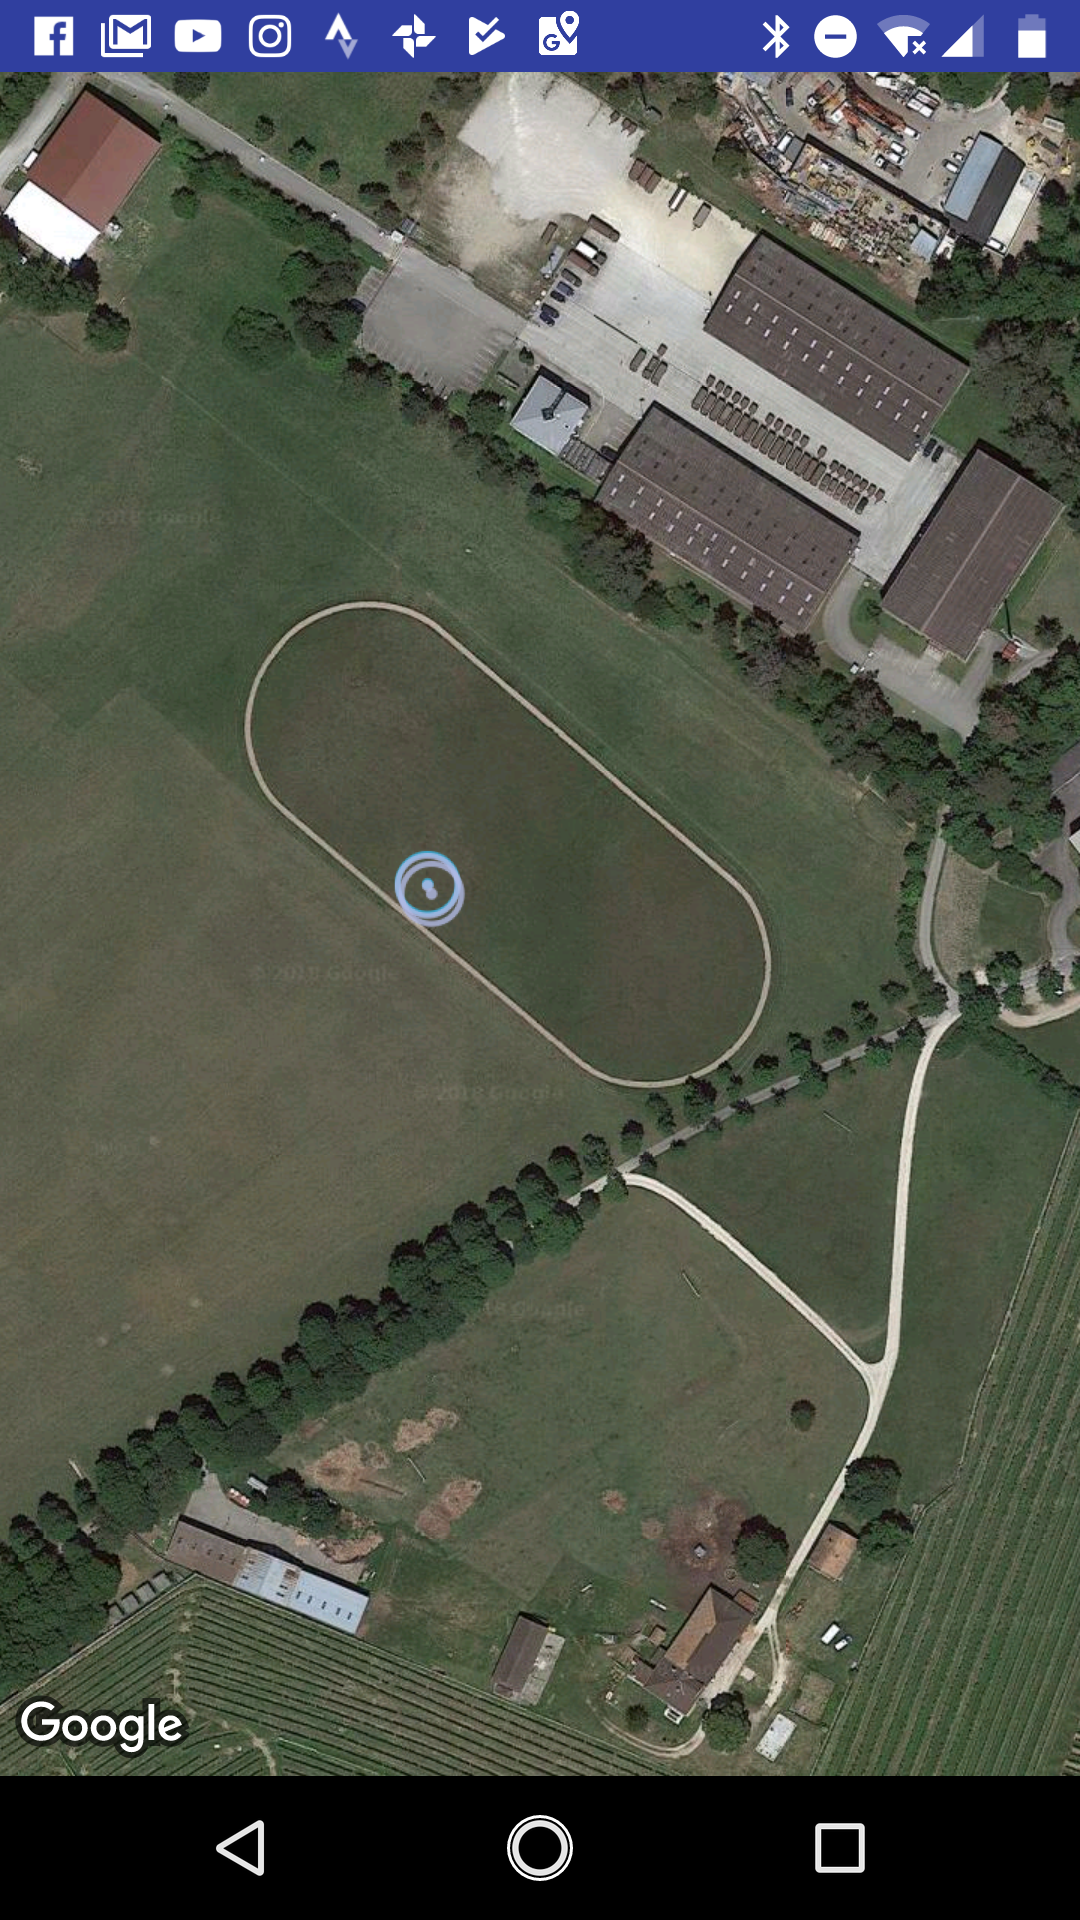
\includegraphics[width=.8\linewidth]{test_2_track1.png}
  \caption{Test \#2 - Image \#1}
  \label{fig:test_2_track1}
\end{subfigure}%
\begin{subfigure}{.5\textwidth}
  \centering
  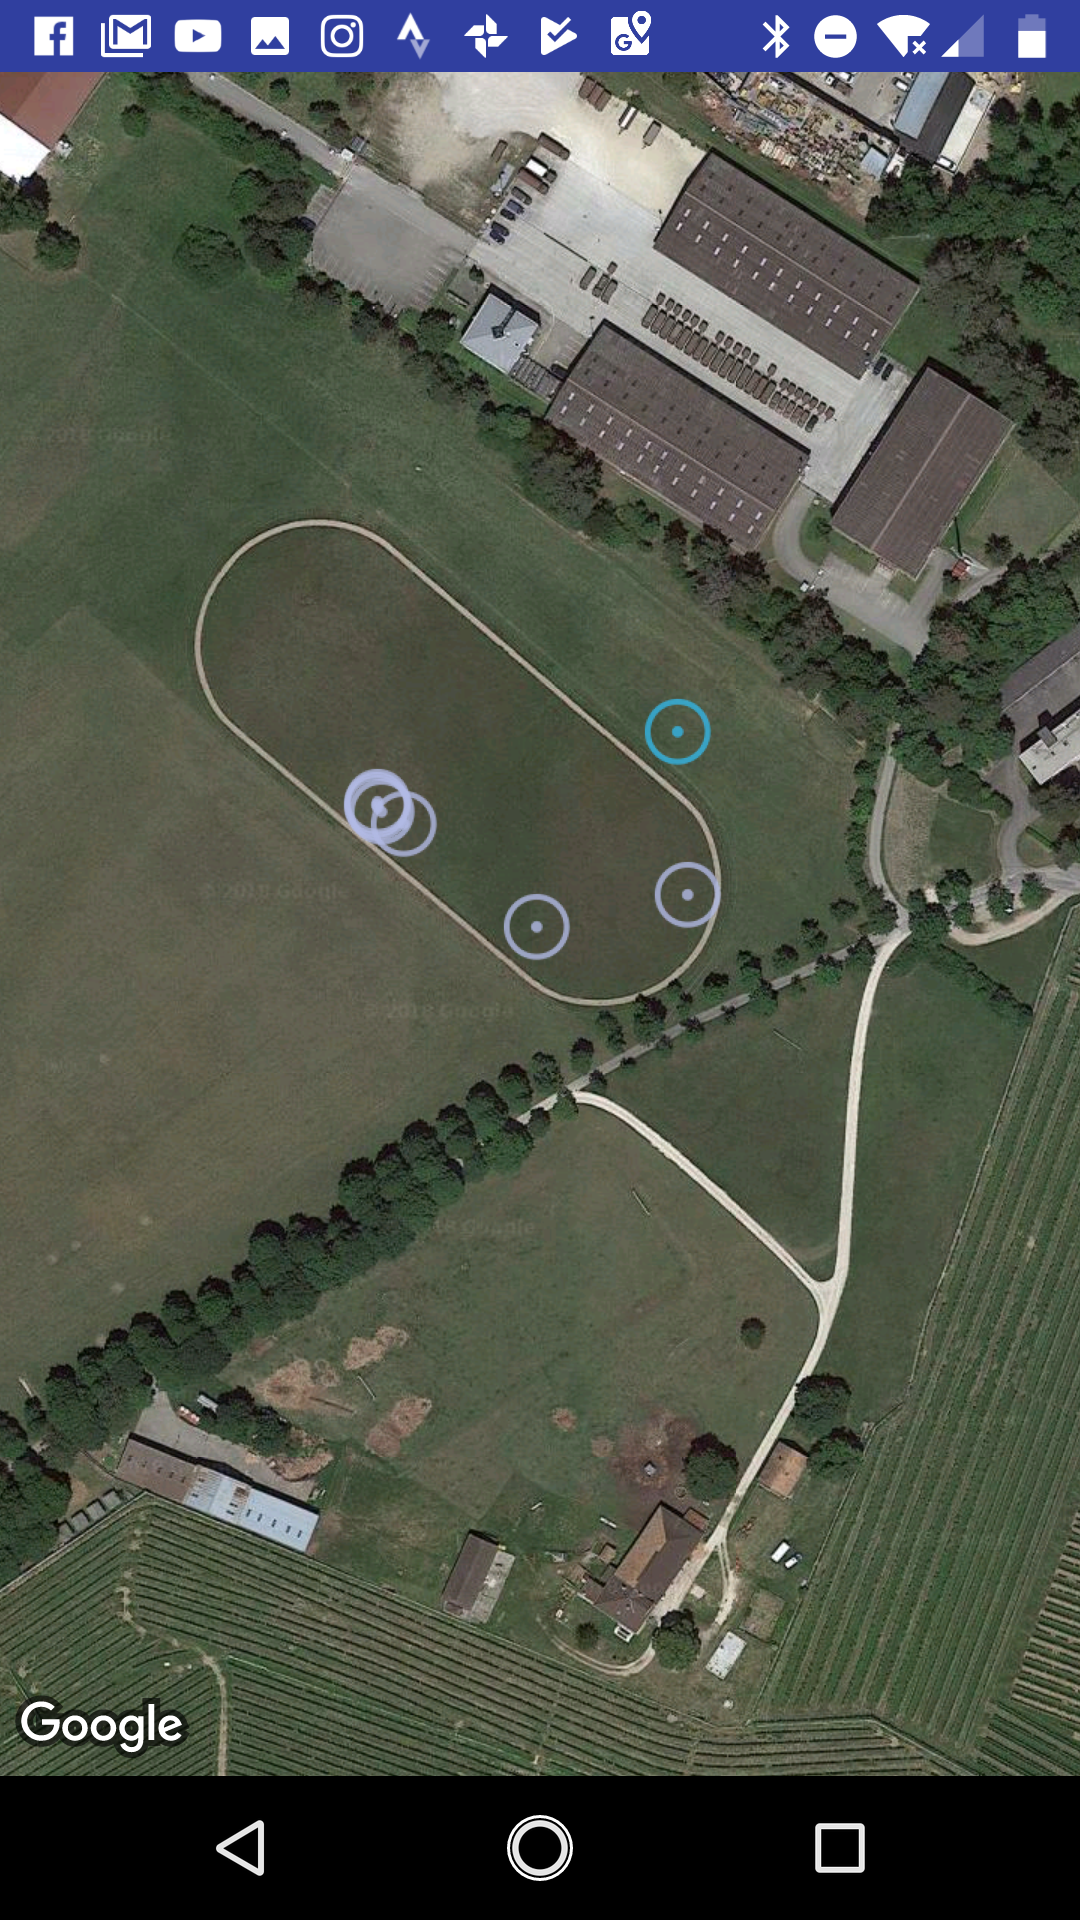
\includegraphics[width=.8\linewidth]{test_2_track2.png}
  \caption{Test \#2 - Image \#2}
  \label{fig:test_2_track2}
\end{subfigure}
\begin{subfigure}{.5\textwidth}
  \centering
  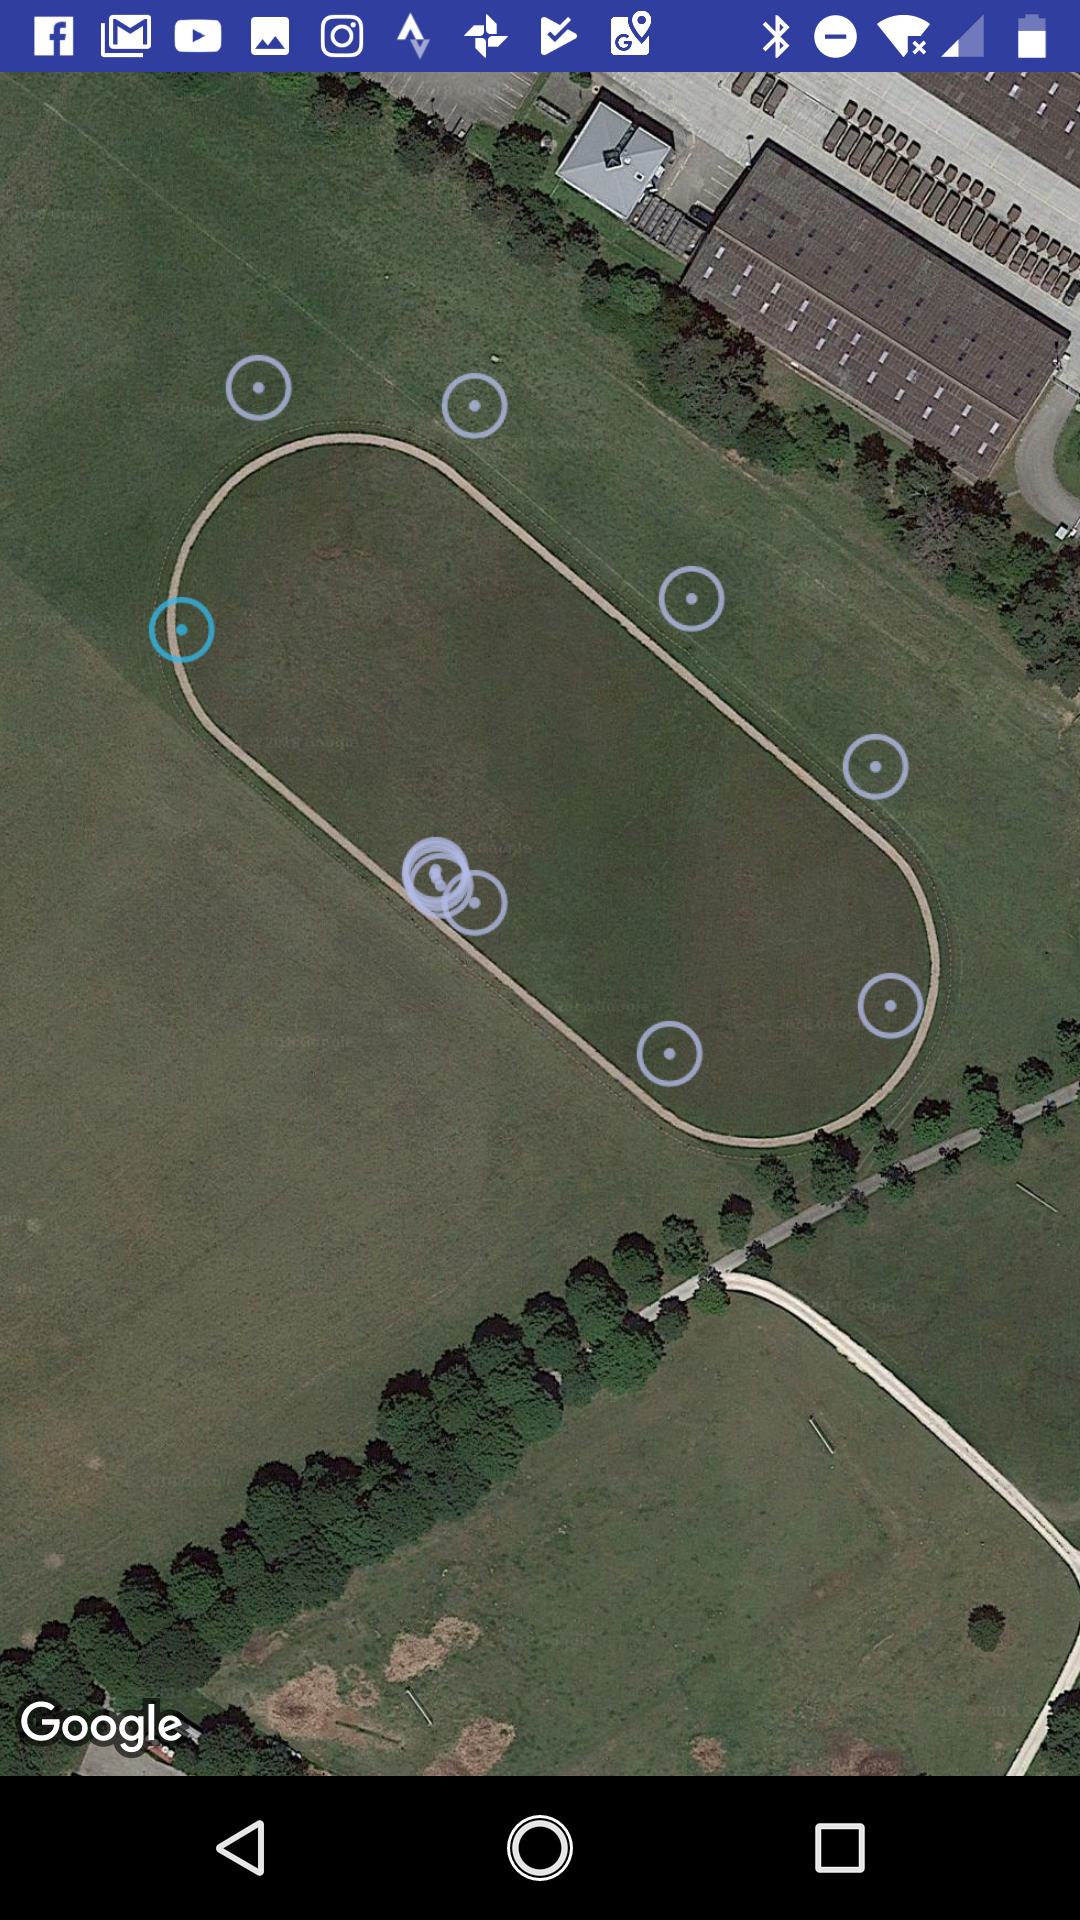
\includegraphics[width=.8\linewidth]{test_2_track3.png}
  \caption{Test \#2 - Image \#3}
  \label{fig:test_2_track3}
\end{subfigure}%
\begin{subfigure}{.5\textwidth}
  \centering
  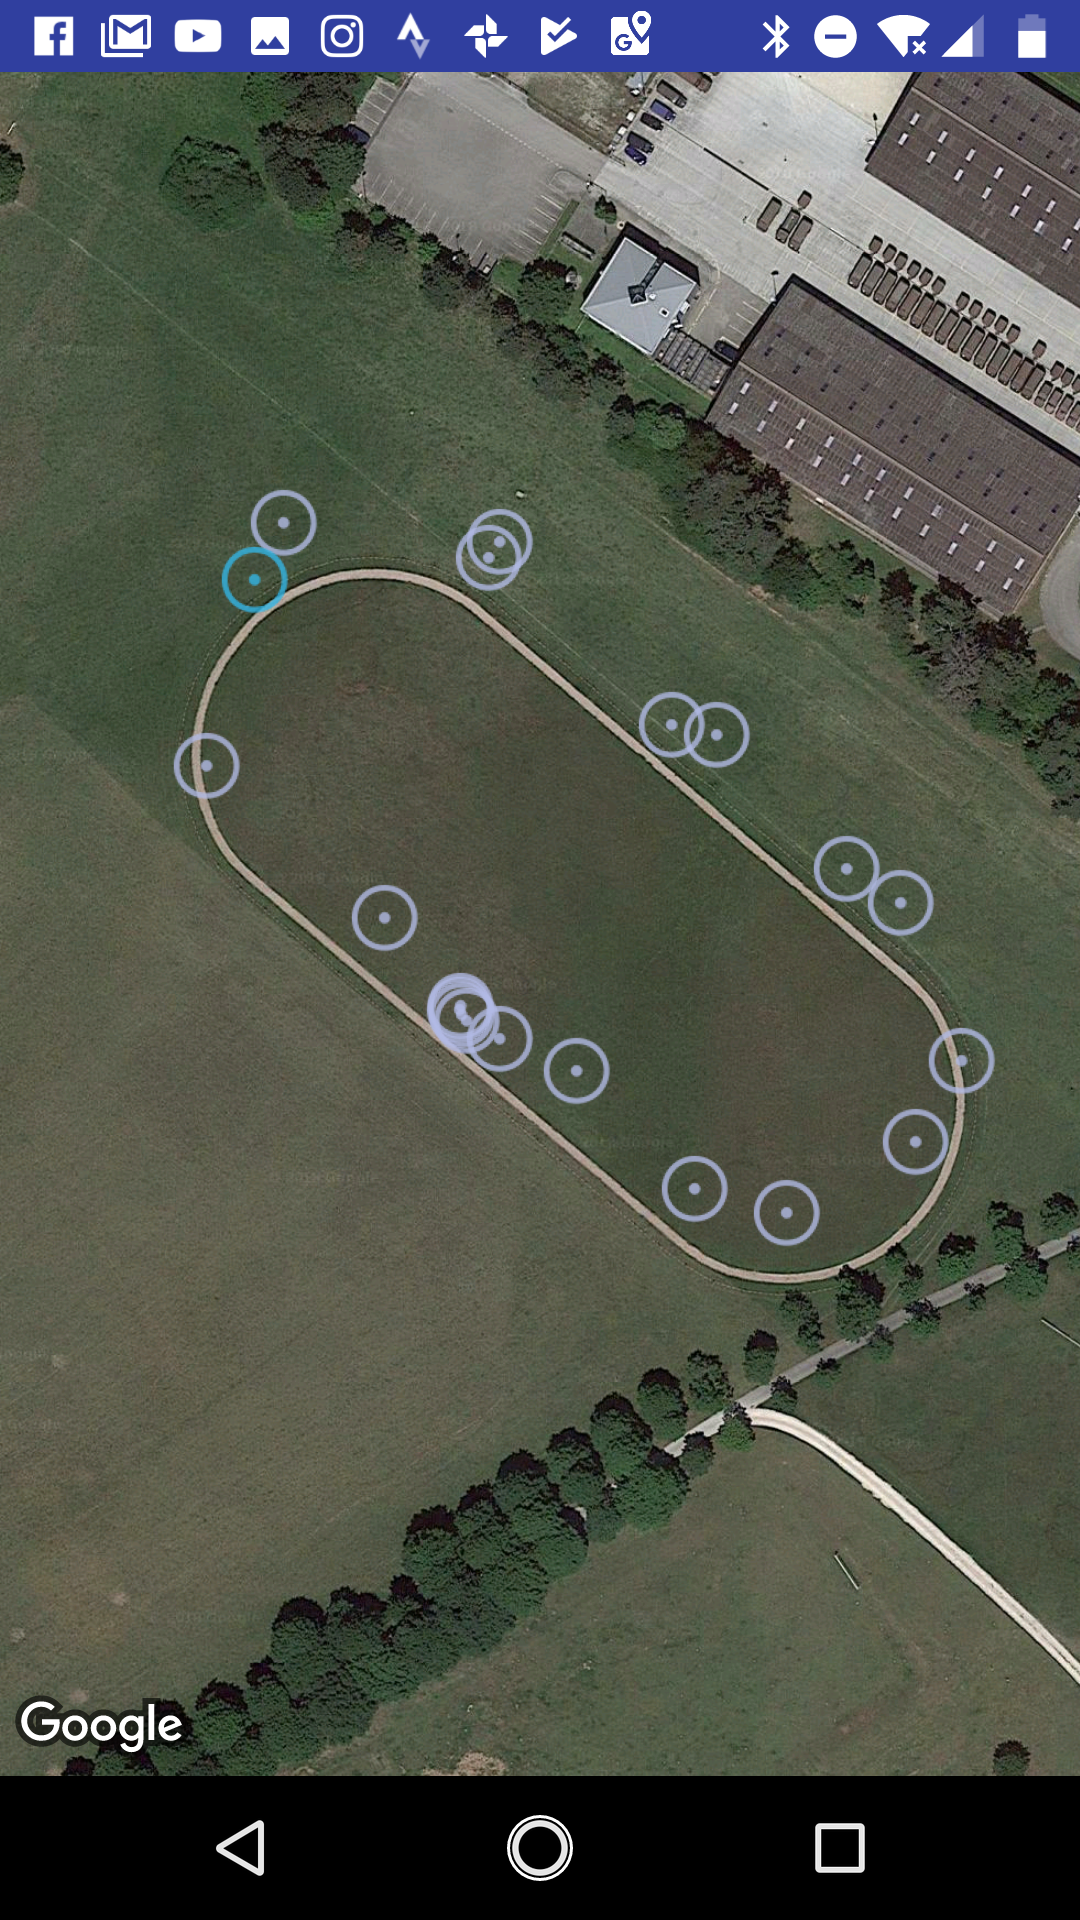
\includegraphics[width=.8\linewidth]{test_2_track4.png}
  \caption{Test \#2 - Image \#4}
  \label{fig:test_2_track4}
\end{subfigure}
\caption{Visualisation des positions reçues du capteur depuis l'application mobile}
\label{fig:test_2}
\end{figure}

\section{Conclusions}

On remarque que les positions reportées sur la carte ne semblent pas être alignées avec la piste. Après des investigations, ceci est dû à un bug au niveau de l'affichage des marqueurs sur la carte. En effet, la position est appliquée à partir du milieu inférieur de l'image, ce qui fait que l'icône n'est pas bien aligné. Après correction du bug les positions sont correctement affichées.

Le test phase \#2 a permis de s'assurer que les positions GPS acquises et transmises dans des paquets LoRa avec le firmware Zephyr permettent d'avoir des précisions très similaires à celle constatées durant le test phase \#1 qui utilisait un logiciel écrit avec le framework Arduino. De manière générale, aucune grosse surprise n’a été révélée par ce test, les performances sont très satisfaisantes également lorsque le porteur du capteur court, ce qui est très encourageant pour la suite du développement du projet.

On peut constater que les données reçues par la passerelle dans les paquets LoRa, leur extraction et stockage fonctionnent conformément aux attentes. La façon d'accéder à la base de données depuis l'application mobile est également validée, à savoir la connexion à l'access point proposé par la passerelle puis l’envoi des requêtes à la base. Aucun problème n’a été mis en lumière de ce côté-là.

Grâce aux résultats du test, on peut conclure que le concept du système de base est parfaitement fonctionnel et qu'aucun problème majeur n’a été révélé durant l'exécution du test. Cela permet donc de valider le développement de la phase \#2 et de passer à la phase suivante qui consiste en la finalisation du système dans son ensemble avec l'implémentation de toutes les fonctionnalités restantes.
